%   Filename    : chapter_4.tex 
\chapter{Preliminary Results/System Prototype}
\section{Preliminary Results}
~~~~The state of the current web-based systems of animal rescue centers are straight-forward and simple. It is important to make it as user-friendly as possible so that it would be easier for the users to engage in the system. But simplicity does not always mean the more users would engage on it. Gamification integrates the “human” to the system and is considered in designing that will motivate more users to take part in using the system.

There are general ways in finding out what motivates the user of an animal rescue center, we then use that motivation to drive the users to do certain actions that they would not normally do. The specific motivation for a web-based animal rescue system that we used is a virtual pet that evolves when it will reach a certain level. The way to gain experience points to level up is by doing actions in a typical animal rescue system like donating, adopting, and volunteering. 

\section{System Prototype}

\subsection{Home Page}
\begin{figure}[H]                %-- use [t] to place figure at top, [b] to place at the bottom, [h] for here
	\centering                    %-- use this to center the figure
	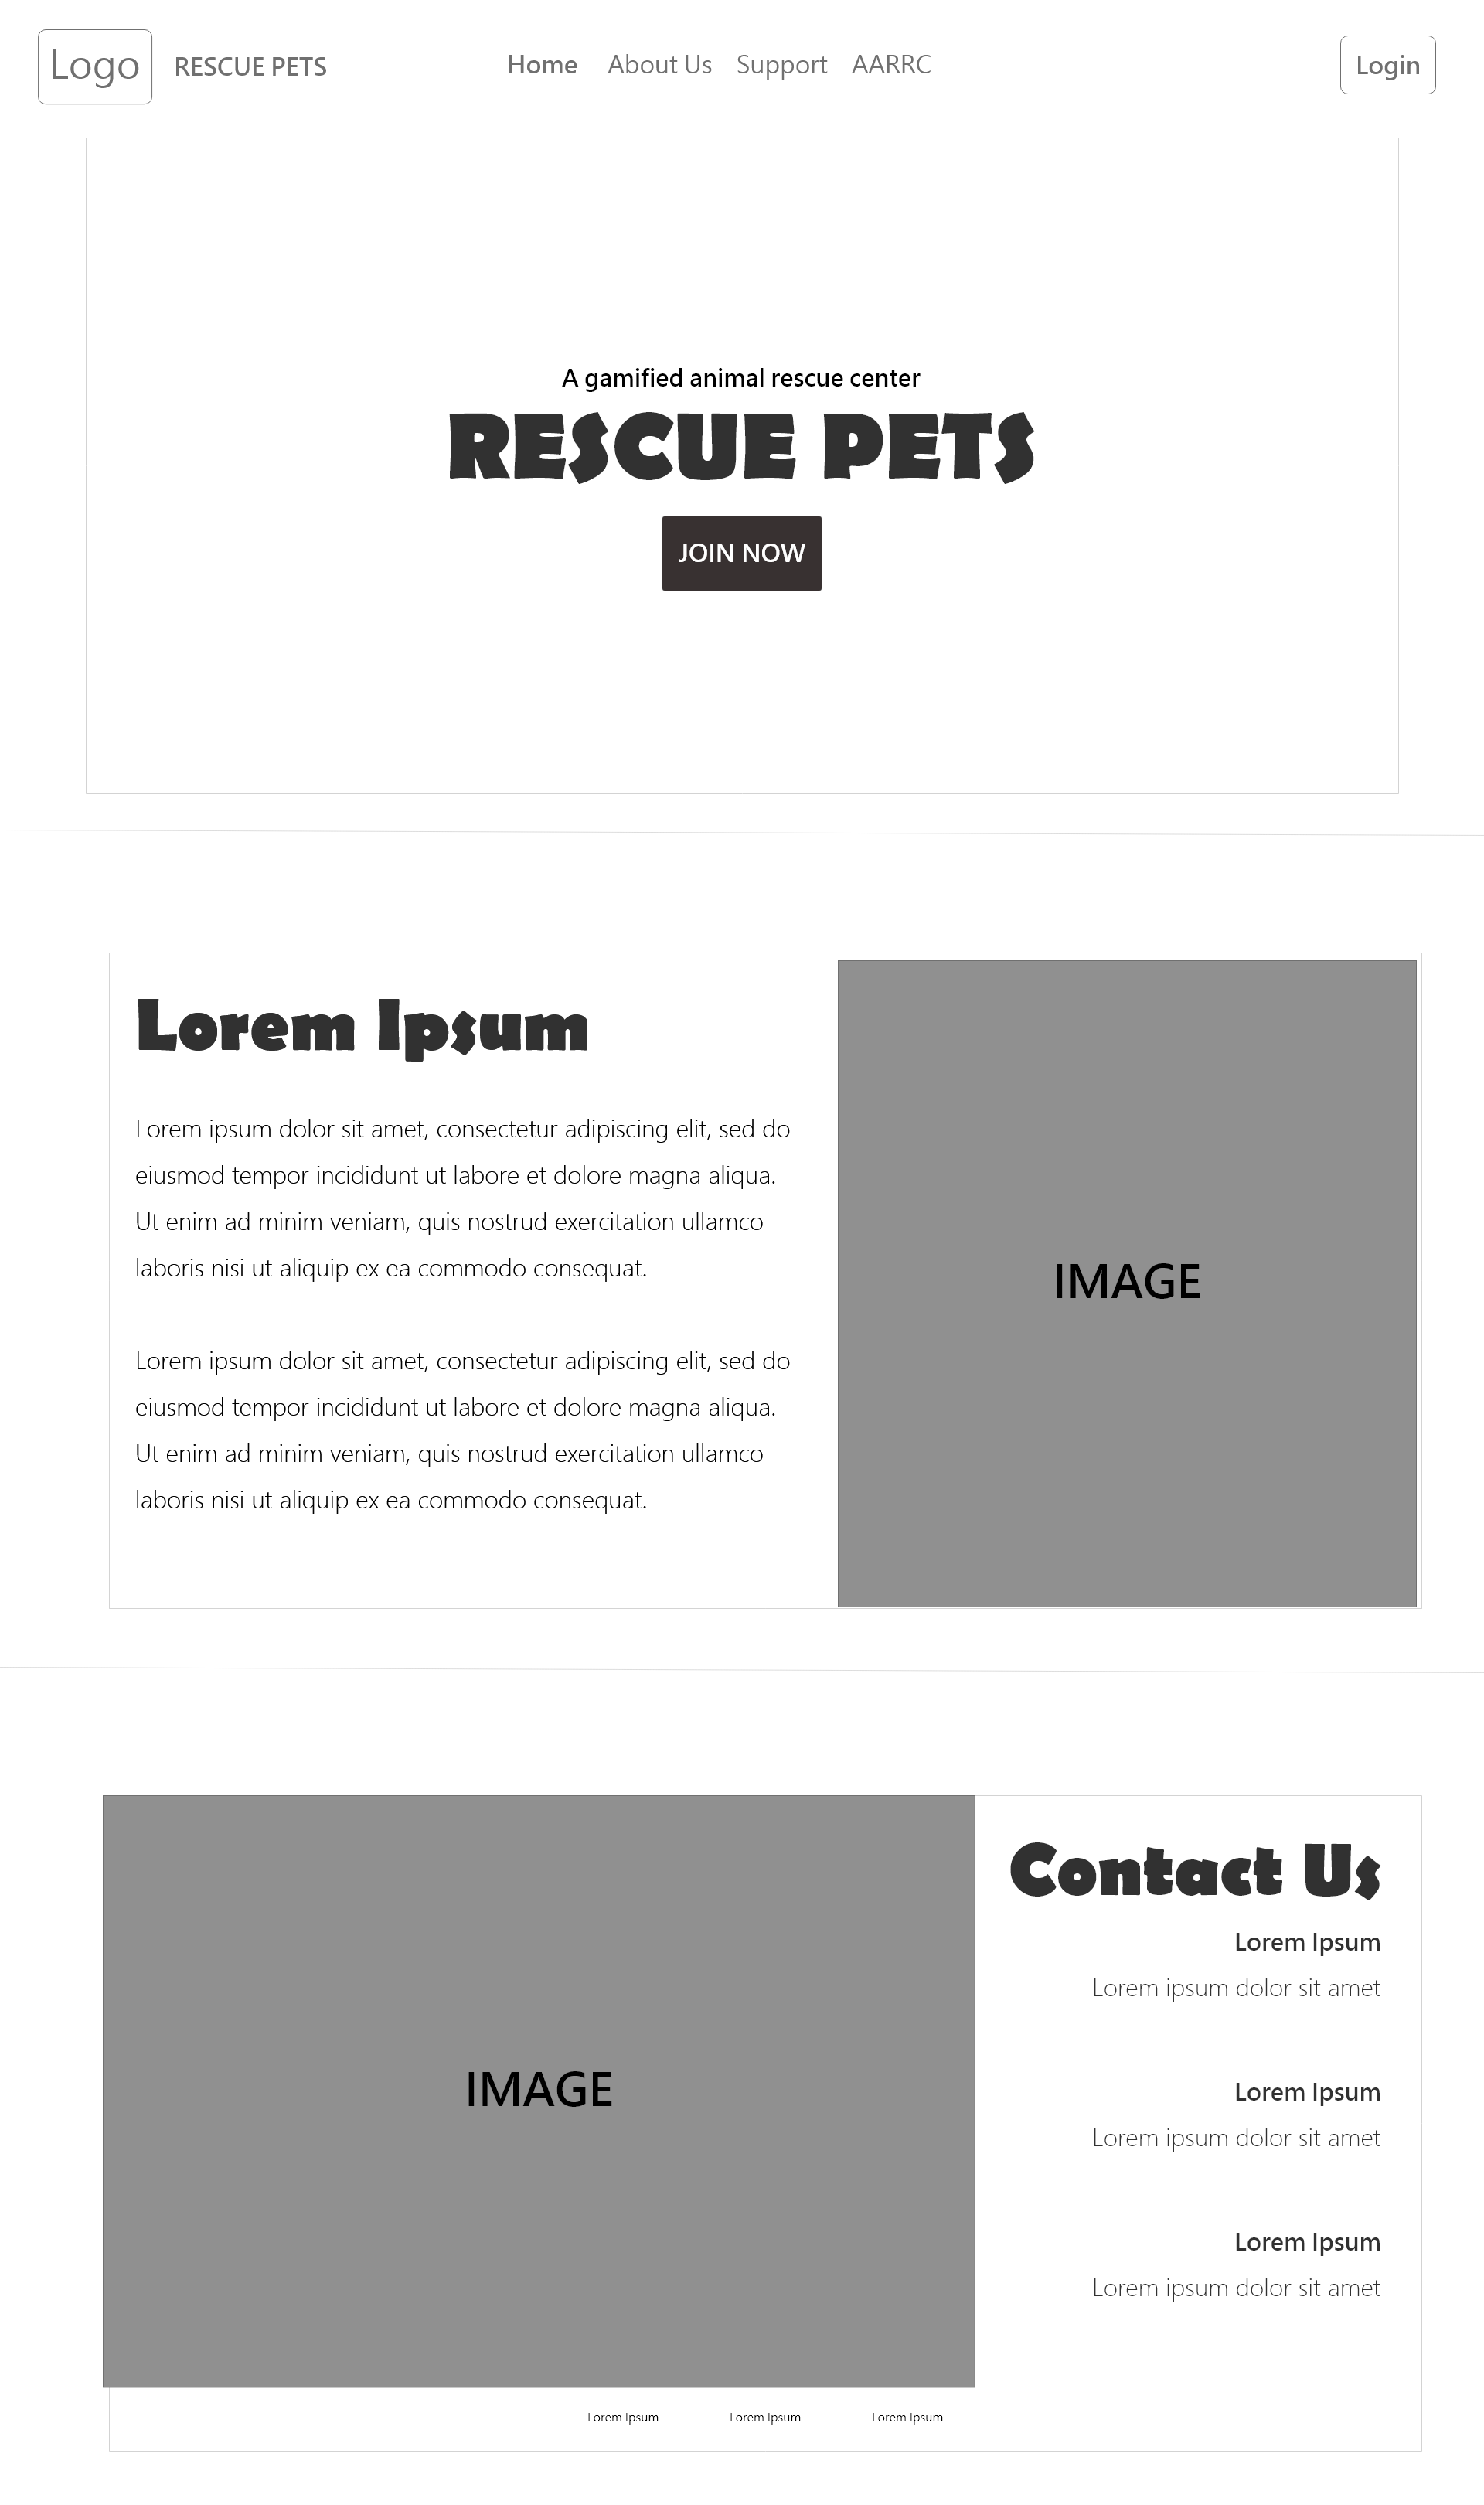
\includegraphics[width=100mm]{Index.png}      %-- include image file named as "disneychart.png" 
	\caption{
		The homepage of the system consists of three sub-pages: the main page, the information page, and the contacts page. Each page can be accessed either by scrolling or aside clicking each corresponding button at the navigation bar above the home page. In the navigation bar. The main page has a “Join Now” button where users can create an account and sign up.}
	\label{fig:Index}
\end{figure}

\subsection{Sign Up Page}
\begin{figure}[H]                %-- use [t] to place figure at top, [b] to place at the bottom, [h] for here
	\centering                    %-- use this to center the figure
	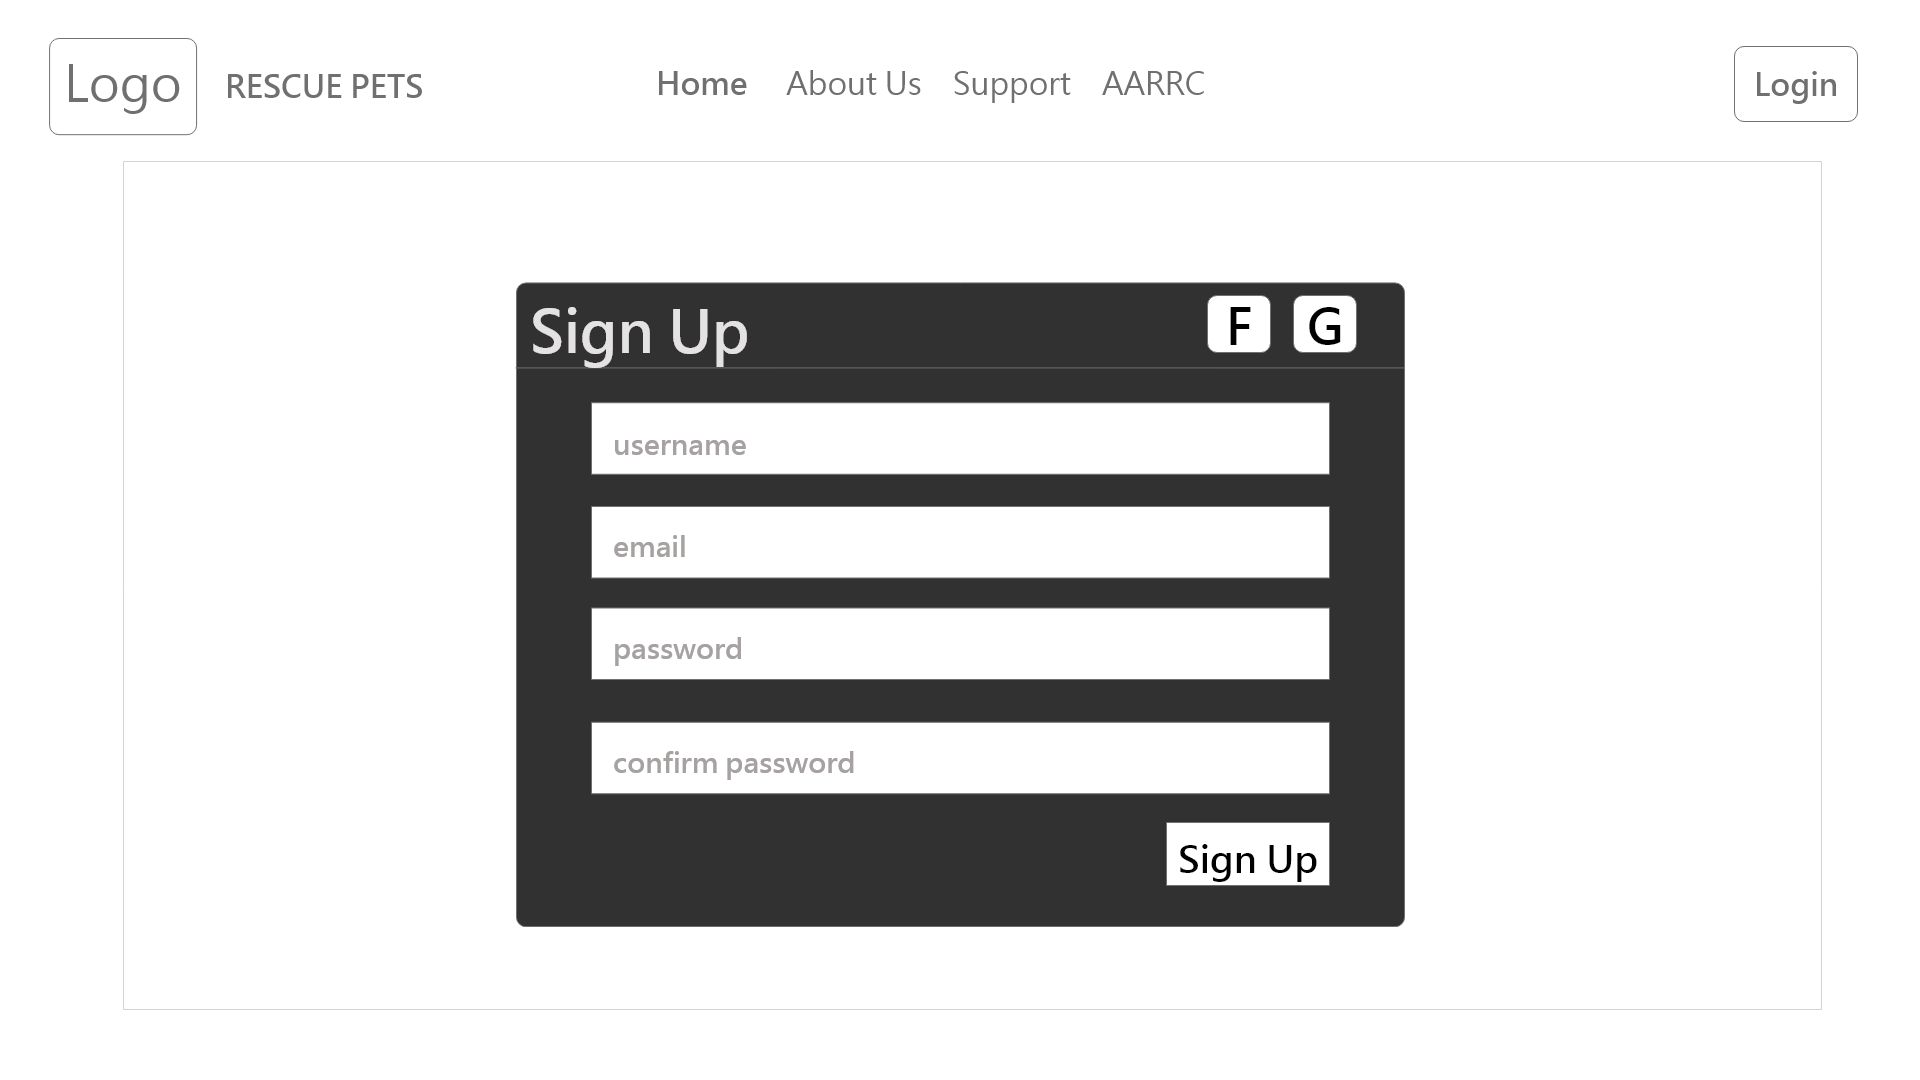
\includegraphics[width=145mm]{Sign_Up.png}      %-- include image file named as "disneychart.png" 
	\caption{
		The sign up page shows a form where the user will input credentials such as username, email, and password. These credentials are used to make an account for the user to access exclusive features such as the virtual pet. The user can also use third-party services to provide necessary information for signing up such as Facebook and Google.}
	\label{fig:Sign_Up}
\end{figure}

\subsection{Navigation Bar}
\begin{figure}[H]                %-- use [t] to place figure at top, [b] to place at the bottom, [h] for here
	\centering                    %-- use this to center the figure
	
\includegraphics[width=145mm]{NavBar.png}      %-- include image file named as "disneychart.png" 
	\caption{
	The navigation bar or the menu bar of the system consists of the brand logo and name, the home link, information link, contacts/support link, and the link to \emph{Aklan Animal Rescue and Rehabilitation Center’s} website, and the Login button where users can input their account credentials to sign in.}
	\label{fig:Navigation}
\end{figure}

\subsection{Log-in Page}
\begin{figure}[H]                %-- use [t] to place figure at top, [b] to place at the bottom, [h] for here
	\centering                    %-- use this to center the figure
	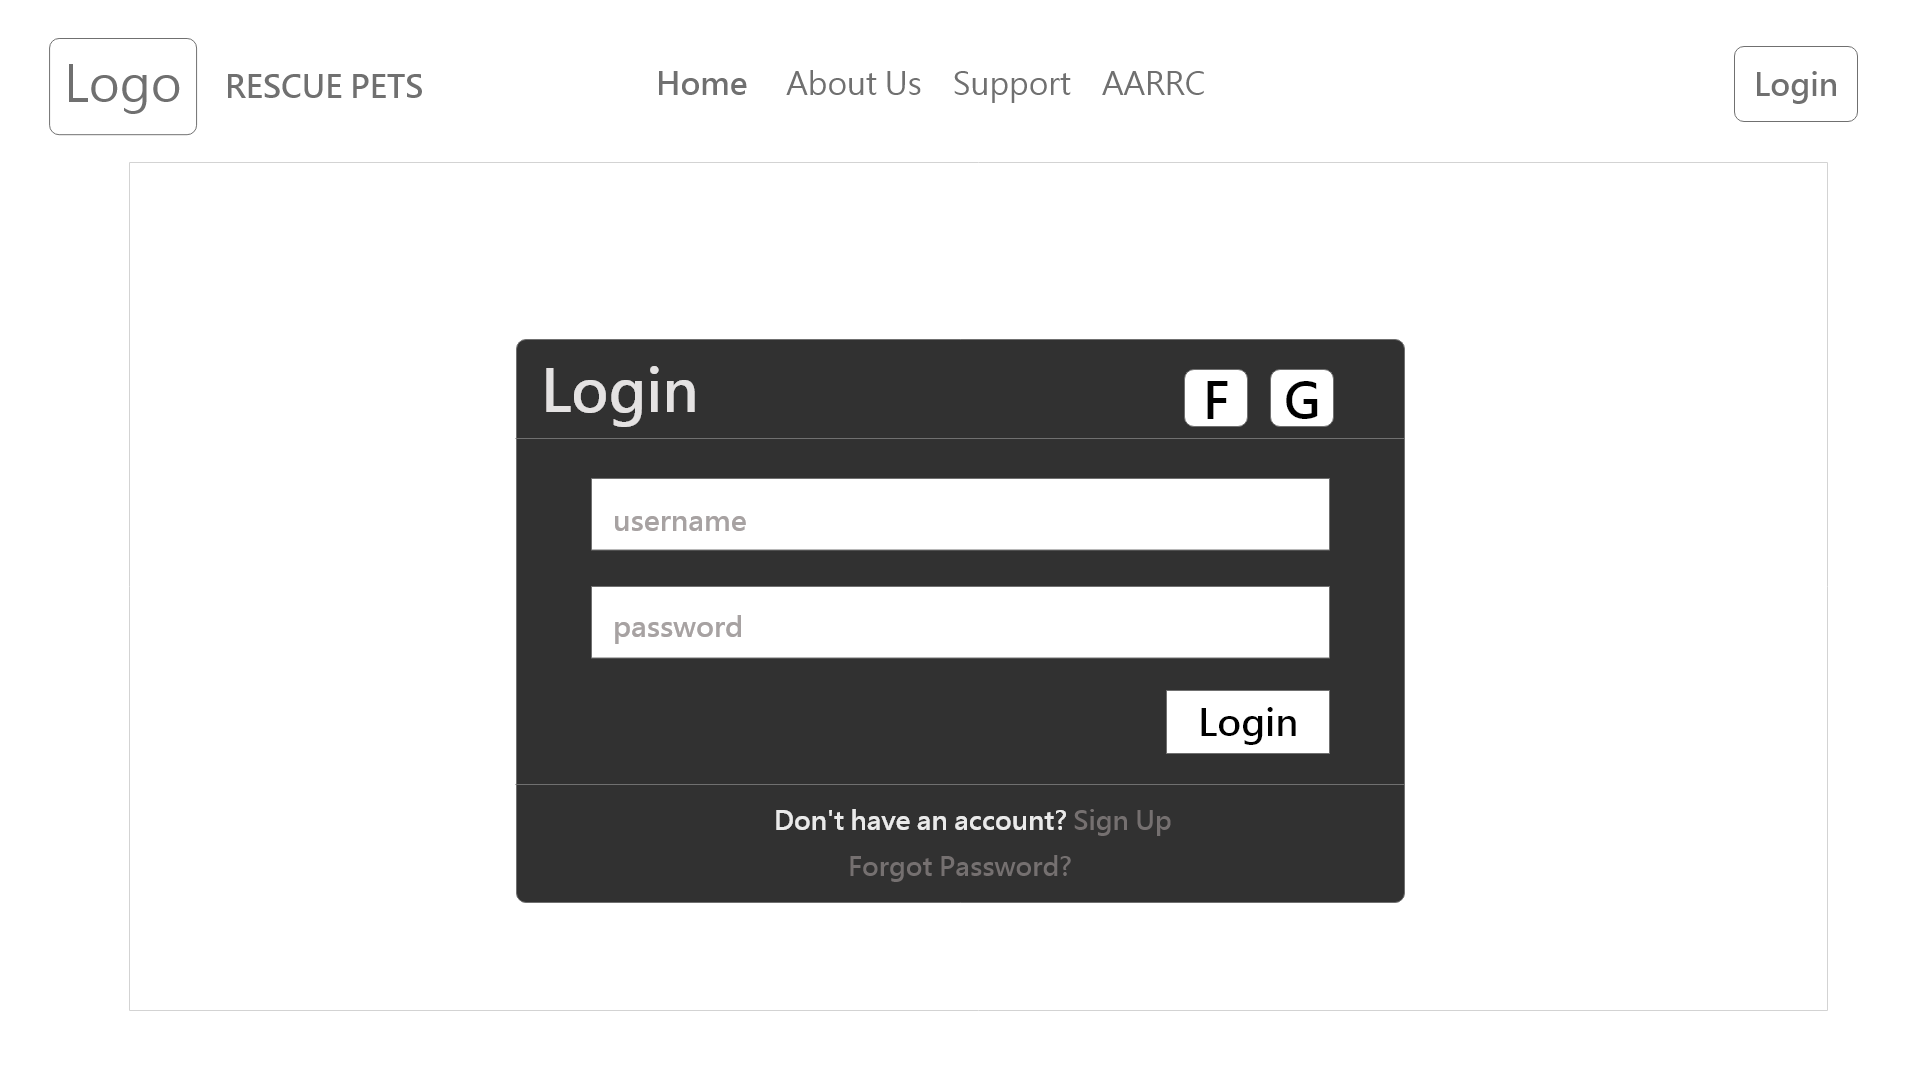
\includegraphics[width=145mm]{Login.png}      %-- include image file named as "disneychart.png" 
	\caption{
	The login page allows the user that has already an existing account to sign in to the system. The user is asked to input the username and password or either use third party services such as Facebook and Google to login.}
	\label{fig:Login}
\end{figure}

\subsection{Profile Page}
\begin{figure}[H]                %-- use [t] to place figure at top, [b] to place at the bottom, [h] for here
	\centering                    %-- use this to center the figure
	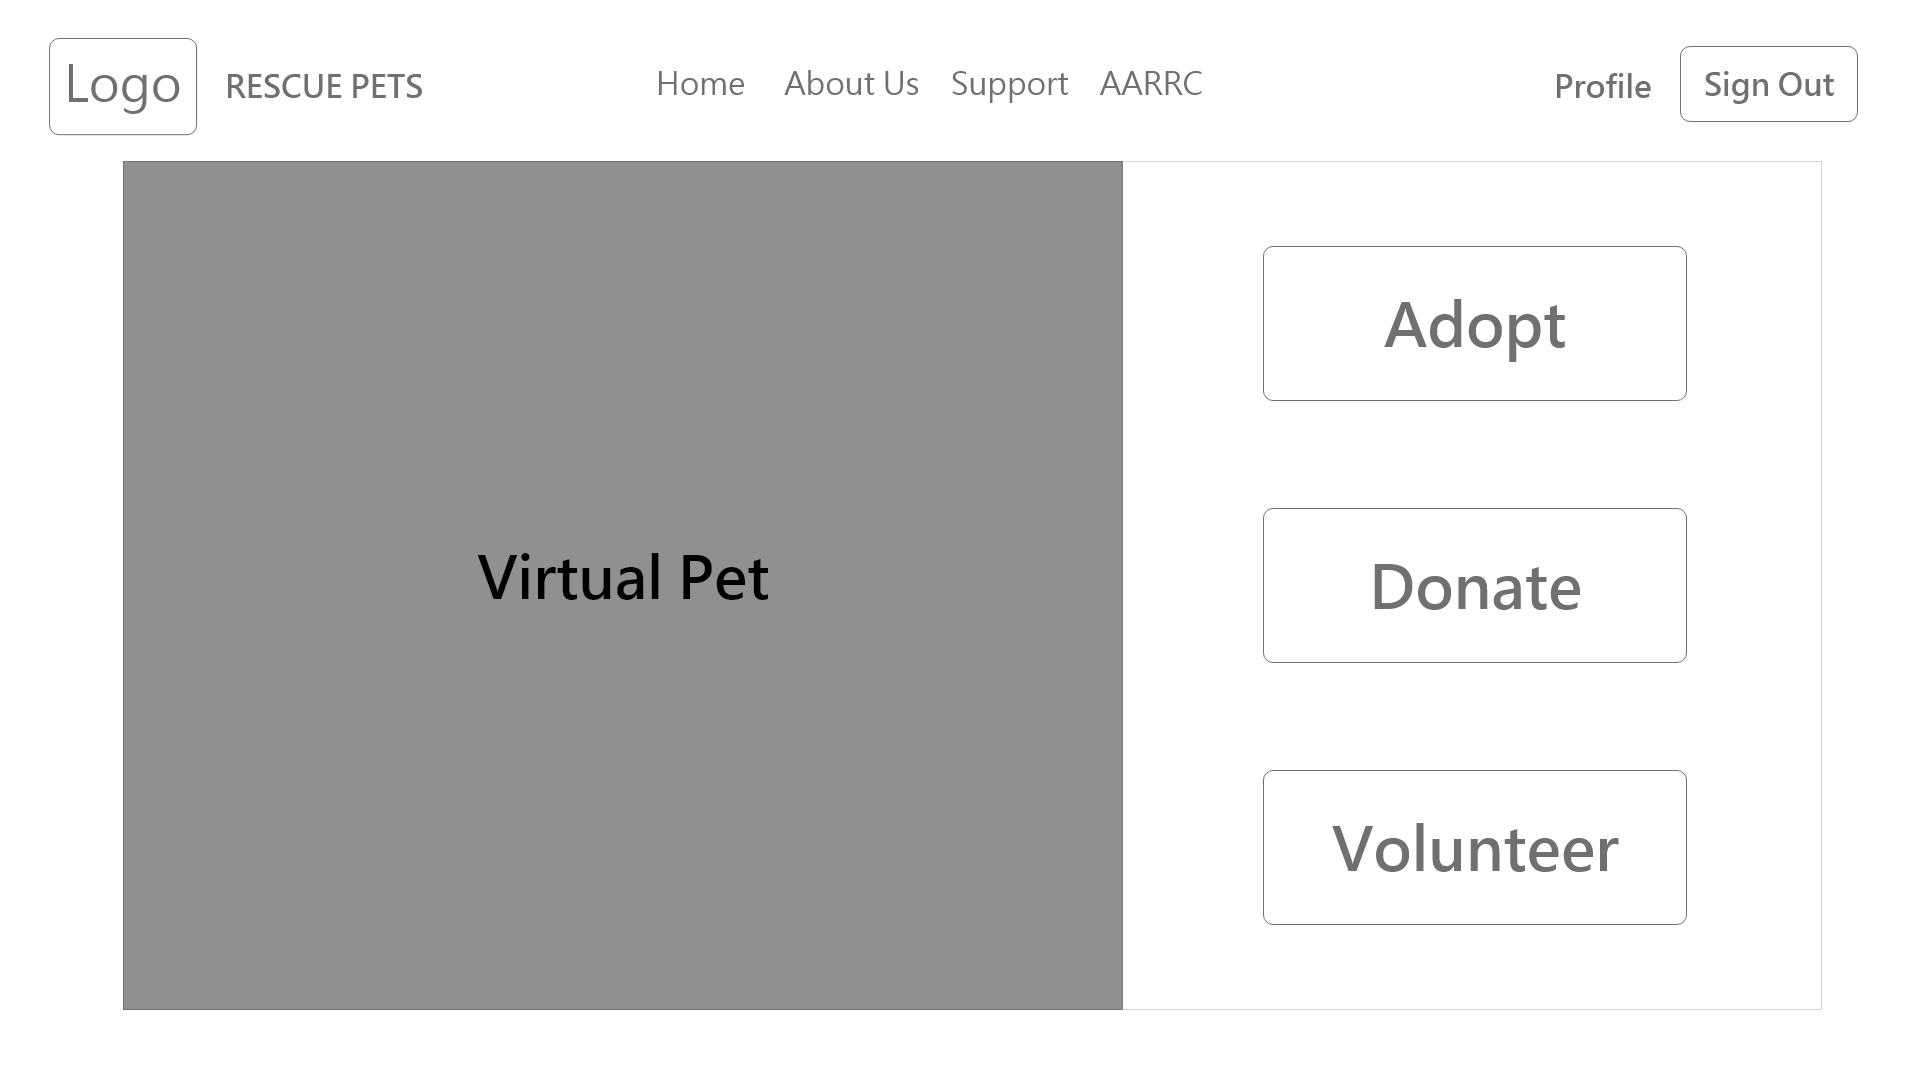
\includegraphics[width=145mm]{Login-Profile.png}      %-- include image file named as "disneychart.png" 
	\caption{
		The user is then greeted by the profile page after logging in to the system. Profile page consists of the user’s virtual pet where information such as level, experience points, and evolution will be shown. It also consists of the adopt, donate, and volunteer button where the user can increase their  virtual pet’s experience point to level up.}
	\label{fig:Login-Profile}
\end{figure}

